\section{Sprint 4 conclusion}\label{sec:sprint4conclusion}
This section concludes sprint 4 and will summarize the progress that has been made on the game and discuss the retrospective meeting conducted at the end of sprint 4.

\subsection{Current product}
The two current states of the game can be seen in \autoref{fig:sprint-4-state-of-game}.
We are currently able to connect to the host in the lobby, as seen on \autoref{fig:sprint-4-lobby}, which will lead to \autoref{fig:sprint-4-game} when the host has started the game.
\begin{figure}[H]
    \centering
    \begin{subfigure}{.5\textwidth}
        \centering
        
\includegraphics[width=1\linewidth]{figures/sprint-4-lobby.PNG}
        \caption{The lobby where you need to input the IP address to connect.}
        \label{fig:sprint-4-lobby}
    \end{subfigure}
    \begin{subfigure}{.4\textwidth}
        \centering
        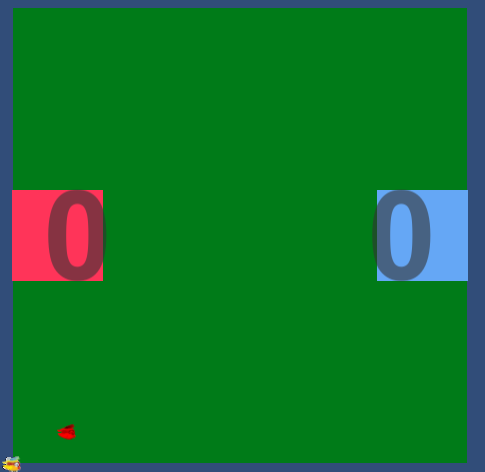
\includegraphics[width=.8\linewidth]{figures/sprint-4-game.PNG}
        \caption{The current playing field with goal zones, goal score and players.}
        \label{fig:sprint-4-game}
    \end{subfigure}
    \caption{The current state of the game}
    \label{fig:sprint-4-state-of-game}
\end{figure}

\subsubsection{Pozyx}
There are not many Pozyx related programming tasks left, but there are some bugs that need to be fixed during the next sprint.
\\
During the initial test of the program described in \autoref{sec:initial-test} several exceptions occurred, which were caused by the input data not being correctly formatted.
This should be fixed in the following sprint.
Problems with the connection were also discovered in the initial test, where Pozyx would not connect to the computer.
Additionally, the tags would occasionally send positional data to the host, with the coordinates of $(0, 0, 0)$.

\subsubsection{Game}
If the problems with Pozyx get fixed, the game should have implemented the majority of the requirements defined for the MVP in \autoref{sec:mvp}.
However, in the current iteration of the game, the teams are unable to win the game.
This is a highly prioritized Unity task, which we intend to implement in the last sprint.

\subsubsection{Networking}
To be able to win the game, it is necessary for the host to be able to send a packet that the game has ended to the clients.
Therefore a packet needs to be specified for this purpose to be implemented along with the ability to win a game.
The host also needs to send information about the number of goals a team needs to score before they win the game, which requires the packet containing player data to be updated to also include goal amount.


\subsection{Retrospective on the process}
This subsection will elaborate on the retrospective meeting that was held on May 12th.

\subsubsection*{How does the process with Jira work?}
The process with Jira will change with the last sprint.
For previous sprints there was a \textit{Suggested} column and a \textit{Discussed} column, but in the upcoming final sprint the \textit{Discussed} column will no longer be used.
Tasks will either be moved to \textit{Chosen for development} or a \textit{Future work} column that was added, rather than go through the \textit{Discussed} column.
The next sprint will be the last, and therefore it is necessary to prioritize it differently.
Either the task has to be completed, or it has to be documented in \textit{Future work}.

\subsubsection*{How has pair programming been working?}
Pair programming works well, but there are some challenges with online pair programming in Unity.
The main challenge is that, when testing, it is required that the game is compiled to an android device, which is more difficult to share with the other programmer unless they both compile the game.

\subsubsection*{How is the daily stand-up working?}
When the members of the group do not have a task, the daily stand up seems pointless, as they do not have much to say.
To change this, at the start of the day the developers should have five minutes to look at possible tasks for the day and pick one, so that they have the opportunity to discuss that during the stand-up meeting.
\\\\
There was also a comment that estimations of completed tasks were inaccurate.
Whenever someone estimated during a stand-up that they would have a task completed by the end of the day, it would often not be completed in time for the next stand-up.
The developer would then give the same estimation, saying it would now be done by the end of the day, and the pattern could repeat.
In order to remedy this the developers should have to specify the reasons why they did not complete the tasks, if they exceeded the estimated duration of the tasks given in a stand-up meeting.
It is suspected that a possible cause of some of this lazy estimation could be that the motivation for certain tasks might be low, and to help this we will introduce pair report writing for larger report tasks, such that the developer pair can help keep each other accountable.

\subsubsection*{How are the reviews going?}
The group members are now more aware of doing the reviews after it was discussed in \autoref{sec:sprint3conclusion}, so reviews often get done at the same day or in the morning the next day.
